% In this file you should put the actual content of the blueprint.
% It will be used both by the web and the print version.
% It should *not* include the \begin{document}
%
% If you want to split the blueprint content into several files then
% the current file can be a simple sequence of \input. Otherwise It
% can start with a \section or \chapter for instance.

\section{Introduction}

The purpose of this paper is to report on the \emph{Equational Theories Project} (ETP)\footnote{\url{https://teorth.github.io/equational_theories/}}, a pilot project launched\footnote{\url{https://terrytao.wordpress.com/2024/09/25}} in September 2024 to explore new ways to collaboratively work on mathematical research projects using machine assistance. The project goal, in the area of universal algebra, was selected\footnote{The specific mathematical goal was inspired by \href{https://mathoverflow.net/questions/450930}{a MathOverflow question}.} to be particularly amenable to crowdsourced and computer-assisted techniques, while still being of mathematical research interest.

The project achieved its primary goal on 14 April 2025, when the $\num{4694} \times (\num{4694}-1) = \num{22028942}$ implications between the test set of $\num{4694}$ equational laws were completely determined, with proofs or refutations formalized in \emph{Lean}.  This required coordinating the efforts of a large number of participants contributing both human-written formalizations and automatically generated proofs from various computer tools.  In this paper, we report on both the scientific outcomes of the project, as well as the organizational issues that came up with organizing a mathematical project of this scale.

\subsection{Magmas and Equational Laws}

In order to describe the mathematical goals of the ETP, we need some notation. A \emph{magma} $\Magma = (M,\op)$ is a set $M$ (known as the \emph{carrier}) together with a binary operation $\op \colon M \times M \to M$. An \emph{equational law} for a magma, or \emph{law} for short, is an identity involving $\op$ and some formal indeterminates, which we will typically denote using the Roman letters $\x,\y,\z,\w,\uu,\vv$, as well as the formal equality symbol $\formaleq$ in place of the equality symbol $=$ to emphasize the formal nature of the law.

In the ETP, a unique number was assigned to each equational law, via a numbering system that we describe in \Cref{numbering-app}.  For instance, the \emph{commutative law} $\x \op \y \formaleq \y \op \x$ is assigned the equation number \eqref{eq43}, while the \emph{associative law} $(\x \op \y) \op \z \formaleq \x \op (\y \op \z)$ is assigned the equation number \eqref{eq4512}.  A list of all equations referred to by number in this paper is also provided in \Cref{numbering-app}.

A magma $\Magma = (M,\op)$ obeys a law $E$ if the law $E$ holds for all possible assignments of the indeterminate to elements of $M$, in which case we write $\Magma \models E$. Thus, for instance $\Magma \models \Eq{43}$ if one has $x \op y = y \op x$ for all $x,y \in M$.  Note that the formal indeterminate symbols $\x, \y$ in $\Eq{43}$ are now replaced by concrete elements $x,y$ of the carrier $M$.

We say that a law $E$ \emph{entails} or \emph{implies} another law $E'$ if every magma that obeys $E$, also implies $E'$: $(\Magma \models E) \implies (\Magma \models E')$.  We write this relation as $E \vdash E'$. We say that two laws are \emph{equivalent} if they entail each other. For instance, the constant law $\x \op \y \formaleq \z \op \w$ \eqref{eq46} can easily be seen to be equivalent to the law $\x \op \x \formaleq \y \op \z$ \eqref{eq41}.  It is clear that $\vdash$ is a pre-order, that is to say a partial order after one quotients by equivalence.

In this entailment pre-ordering, the maximal element is given by the trivial law $\x\formaleq\x$ \eqref{eq1}, and the minimal element is given by the singleton law $\x\formaleq \y$ \eqref{eq2}, thus $\Eq{2} \vdash E \vdash \Eq{1}$ for all laws $E$.

We also define a variant: we say that $E$ \emph{entails} $E'$ \emph{for finite magmas}, and write $E \vdashfin E'$, if every \emph{finite} magma $M$ that obeys $E$, also obeys $E'$.  Clearly, the relation $E \vdash E'$ implies $E \vdashfin E'$; but, as observed by Austin \cite{austin_finite}, the converse is not true in general.

The \emph{order} of an equational law is the number of occurrences of the magma operation, and can be viewed as a crude measure of complexity of the law. For instance, the commutative law \eqref{eq43} has order $2$, while the associative law \eqref{eq4512} has order $4$. We note some selected laws of small order that have previously appeared in the literature:
\begin{itemize}
\item The \emph{central groupoid law} $\x \formaleq (\y \op \x) \op (\x \op \z)$ \eqref{eq168} is an order-$3$ law introduced by Evans \cite{evans} and studied further by Knuth \cite{knuth} and many further authors, being closely related to central digraphs (also known as unique path property digraphs), and leading in particular to the discovery of the Knuth-Bendix algorithm \cite{knuth-bendix}; see \cite{klt} for a more recent survey.
\item \emph{Tarski's axiom} $\x \formaleq \y \op (\z \op (\x \op (\y \op \z)))$ \eqref{eq543} is an order-$4$ law that was shown by Tarski \cite{Tarski1938} to characterize the operation of subtraction in an abelian group; that is to say, a magma $\Magma = (M,\op)$ obeys \eqref{eq543} if and only if there is an abelian group structure on $\Magma$ for which $x \op y = x-y$ for all $x,y \in M$.
\item In a similar vein, it was shown in \cite{mendelsohn-padmanabhan} (see also \cite{meredith-prior}) that the order-$4$ law
$\x \formaleq (\y \op \z) \op (\y \op (\x \op \z))$ \eqref{eq1571} characterizes addition (or subtraction) in an abelian group of exponent $2$; it was shown in \cite{mccune_et_al} that the order-$6$ law $\x \formaleq (\y \op ((\x \op \y) \op \y)) \op (\x \op (\z \op \y))$ \eqref{eq345169} characterizes the Sheffer stroke in a boolean algebra, and it was shown in \cite{higman-neumann} that the order-$8$ law
$\x \formaleq \y \op ((((\y \op \y) \op \x) \op \z) \op (((\y \op \y) \op \y) \op \z))$ \eqref{eq42323216} characterizes division in a (not necessarily abelian) group.
\end{itemize}
Some further examples of laws characterizing well-known algebraic structures are listed in \cite{mccune-survey}.

The Birkhoff completeness theorem \cite[Th.~3.5.14]{term-rewriting} implies that an implication $E \vdash E'$ of equational laws holds if and only if the left-hand side of $E'$ can be transformed into the right-hand side by a finite number of substitution rewrites using the law $E$. However, the problem of determining whether such an implication holds is undecidable in general \cite{mckenzie}. Even when the order is small, some implications\footnote{Another contemporaneous example of this phenomenon was the solution of the Robbins problem \cite{robbins}.} can require lengthy computer-assisted proofs; for instance, it was noted in \cite{Kisielewicz2} that the order-$4$ law $\x \formaleq (\y \op \x) \op ((\x \op \z) \op \z)$ \eqref{eq1689} was equivalent to the singleton law \eqref{eq2}, but all known proofs were found with computer assistance.\footnote{We improved such a proof to make it human-readable, see \href{https://teorth.github.io/equational_theories/blueprint/implications-chapter.html}{the blueprint of the ETP}.}  Furthermore, for the finite magma implication relation $E \vdashfin E'$, no analogue of the Birkhoff completeness theorem is available.

\subsection{The Equational Theories Project}

As noted in \Cref{numbering-app}, there are $\num{4694}$ equational laws of order at most $4$. The primary mathematical goal of the ETP was to completely determine the \emph{implication graph} for these laws, in which there is a directed edge from $E$ to $E'$ precisely when $E \vdash E'$. As the project progressed, an additional goal was added to determine the slightly larger \emph{finite implication graph}, in which there is a directed edge from $E$ to $E'$ precisely when $E \vdashfin E'$.

Such systematic determinations of implication graphs have been seen previously in the literature; for instance, in \cite{phillips-vojtechovsky}, the relations between $60$ identities of Bol--Moufang type were established, and in the blog post \cite[\S 17]{Wolfram_2022}, some initial steps towards generating this graph for the first hundred or so laws on our list were performed. However, to our knowledge, the ETP is the first project to study such implications at the scale of thousands of laws.

The ETP requires the determination of the truth or falsity of $\num{4694}^2 = \num{22033636}$ implications (for both arbitrary magmas and finite magmas), or $\num{4694} \times (\num{4694}-1) = \num{22028942}$ if the reflexive implications $E \vdash E$ are removed; while one can use properties such as the transitivity of entailment to reduce the work somewhat, this is clearly a task that requires significant automation. It was also a project highly amenable to crowdsourcing, in which different participants could work on developing different techniques, each of which could be used to fill out a different part of the implication graph. In this respect, the project could be compared with a Polymath project \cite{Gowers2009}, which used online forums such as blogs and wikis to openly collaborate on a mathematical research problem. However, the Polymath model required human moderators to review and integrate the contributions of the participants, which clearly would not scale to the ETP which required the verification of over twenty million mathematical statements. Instead, the ETP was centered around a GitHub repository in which the formal mathematical contributions had to be entered in the proof assistant language \emph{Lean}, where they could be automatically verified. In this respect, the ETP was more similar to the recently concluded Busy Beaver Challenge\footnote{\url{https://bbchallenge.org/}}, which was a similarly crowdsourced project that computed the fifth Busy Beaver number $BB(5)$ to be $\num{47176870}$ through an analysis of about $180$ million Turing machines, with the halting analysis being verified in a variety of computer languages, with the final formal proof written in the proof assistant language \emph{Coq} \cite{the_coq_development_team_2024_14542673, bbchallenge_bb5}. One of the aims of the ETP was to explore potential workflows for such collaborative, formally verified mathematical research projects that could serve as a model for future projects of this nature.

Secondary aims of the ETP included the possibility of discovering unusually interesting equational laws, or new experimental observations about such laws, that had not previously been noticed in the literature; and to develop benchmarks to assess the performance of automated theorem provers and other AI tools.

\subsection{Outcomes}

The ETP achieved almost all of its primary objectives, with all of the $\num{22033636}$ implications $E \vdash E'$ and non-implications $E \not \vdash E'$ magmas formalized in the proof assistant language \emph{Lean}, and can be found on the ETP GitHub repository.  See \Cref{fig:854}, \Cref{fig:1729} and \Cref{fig:longchain} for some small fragments of the implication graphs produced.
The $\num{4694}$ laws organized into $\num{1415}$ equivalence classes, with by far the largest class being the class of $\num{1496}$ equations equivalent to the trivial law $\Eq{2}$.

For the finite implication graph $E \vdashfin E'$, we could similarly formalize all but two implications.  Specifically, we were unable to obtain either a human-readable or formalized proof or disproof of the implication $E677 \vdashfin E255$ (or its equivalent dual $E2910 \vdashfin E47$), despite extensive efforts from the participants of the project; we tentatively conjecture this implication to be false (i.e., that there exists a finite magma obeying \eqref{eq677} but not \eqref{eq255}), but the refutation appears to be ``immune'' to most of the techniques that we developed for the project.  (We were however able to establish that the corresponding implication $E677 \vdash E255$ for arbitrary magmas was false, using the greedy construction discussed in \Cref{greedy-sec}.)

\begin{figure}
\centering
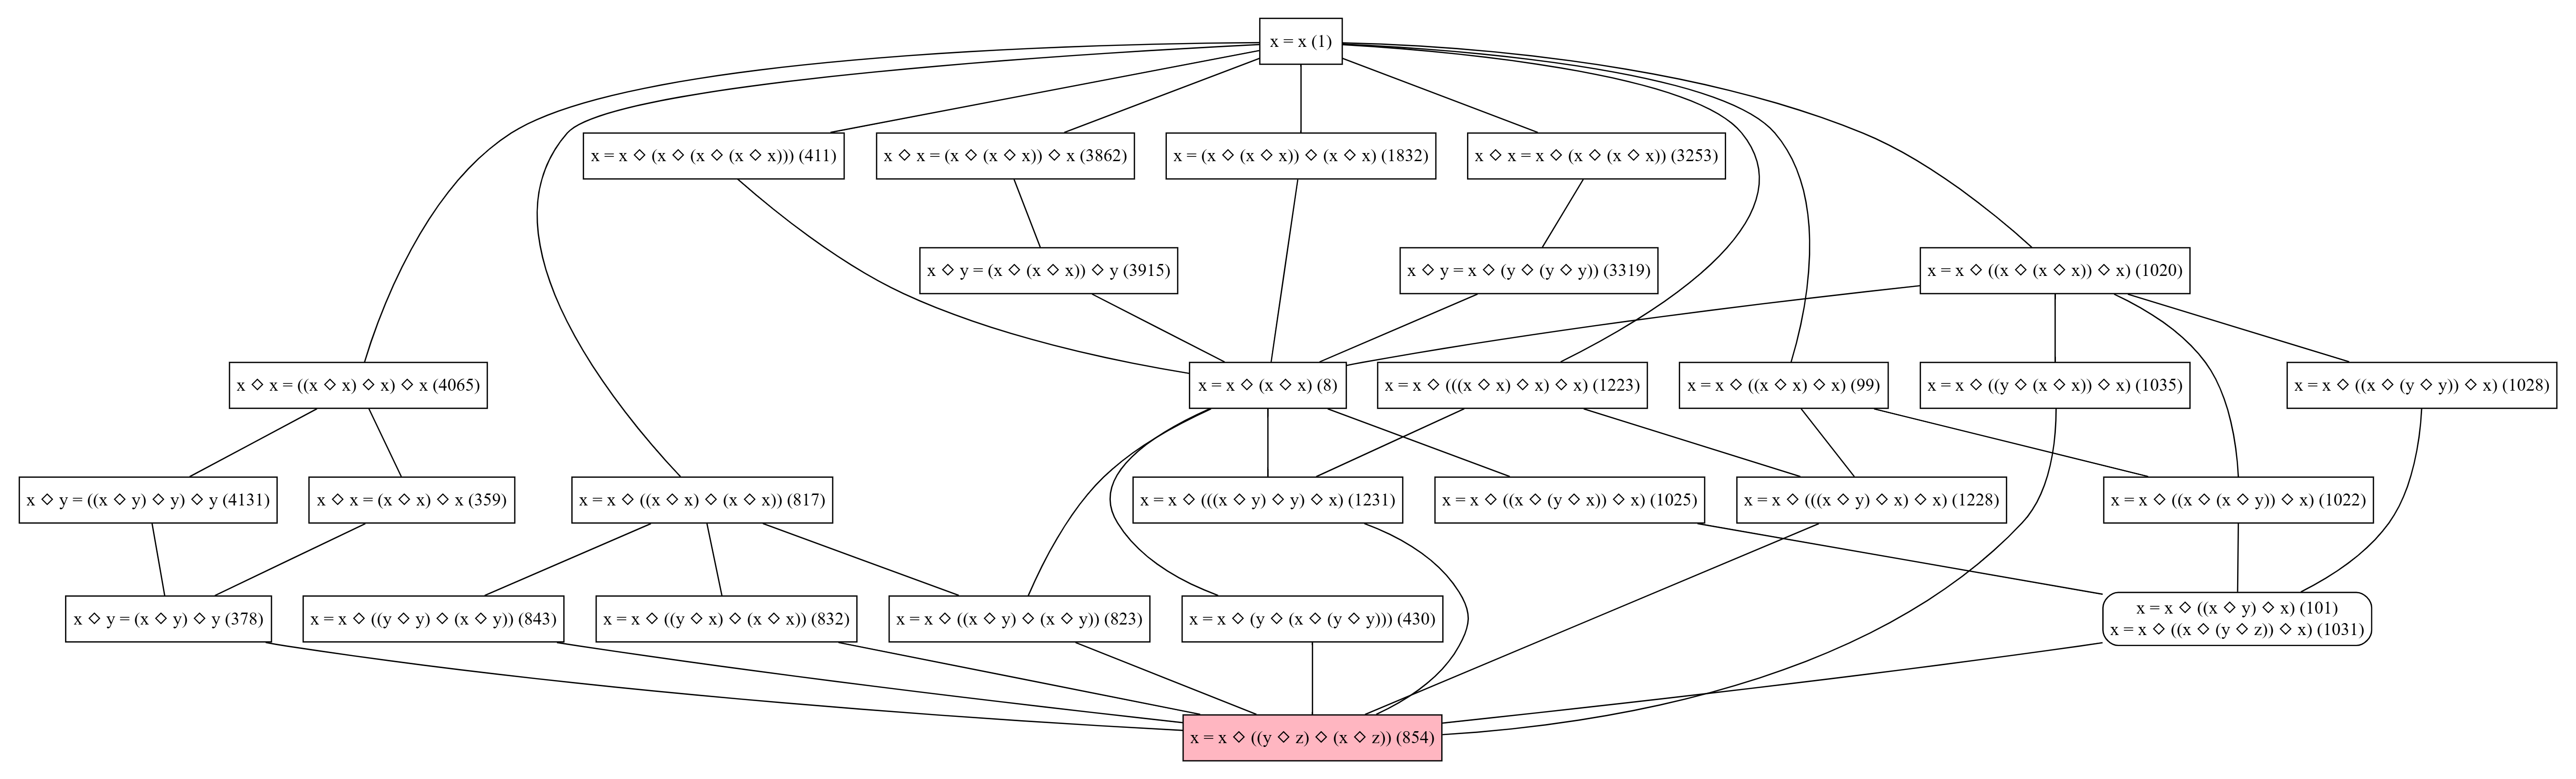
\includegraphics[width=0.85\textwidth]{854.png}
\caption{A Hasse diagram of all the equational laws implied by \eqref{eq854} (for unrestricted magmas).  An edge in this diagram indicates that the lower equation implies the higher one. Rounded rectangles indicate groups of equivalent laws.  This graph was produced by the visualization tool \emph{Graphiti}, which was developed for this project.}
\label{fig:854}
\end{figure}

\begin{figure}
    \centering
    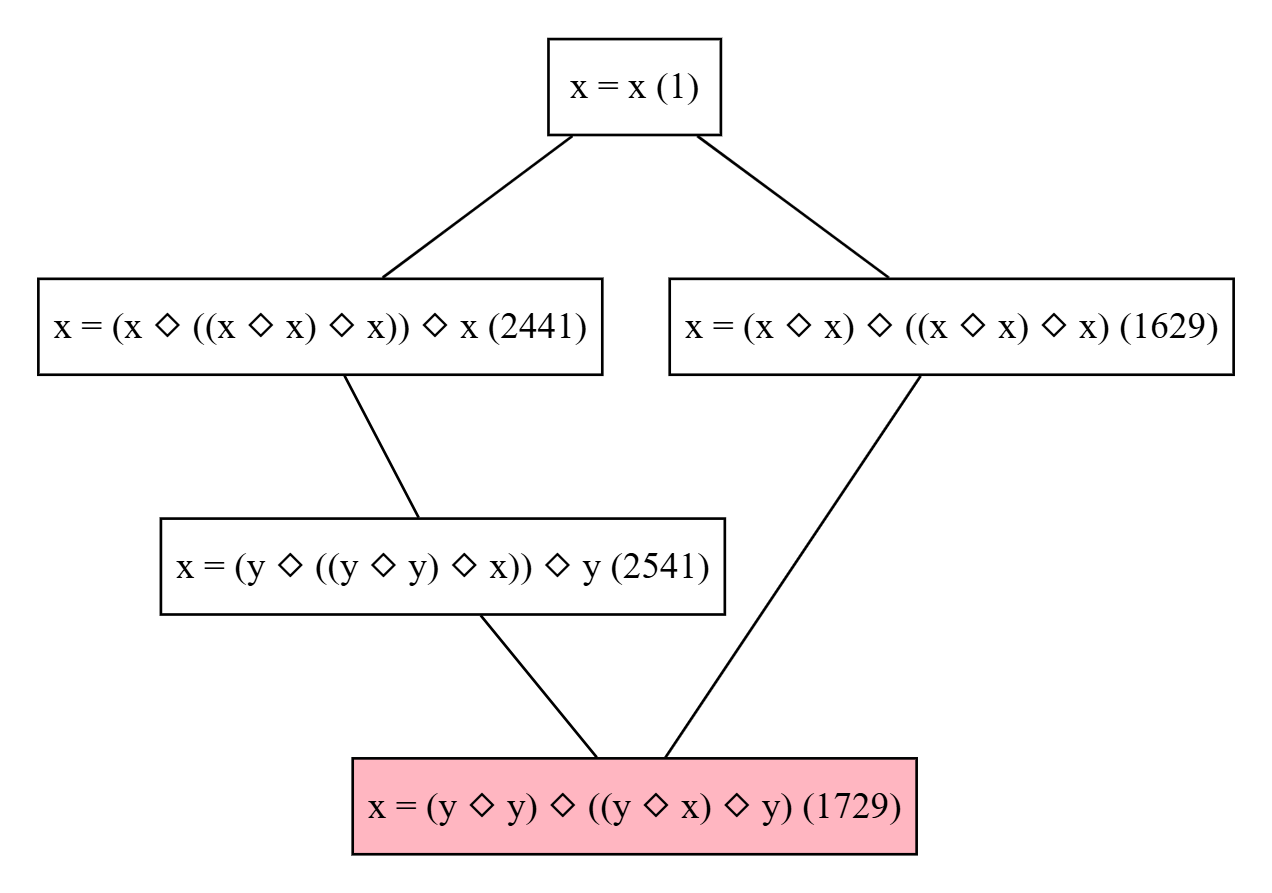
\includegraphics[width=0.4\textwidth]{ramanujan-infinite.png}
    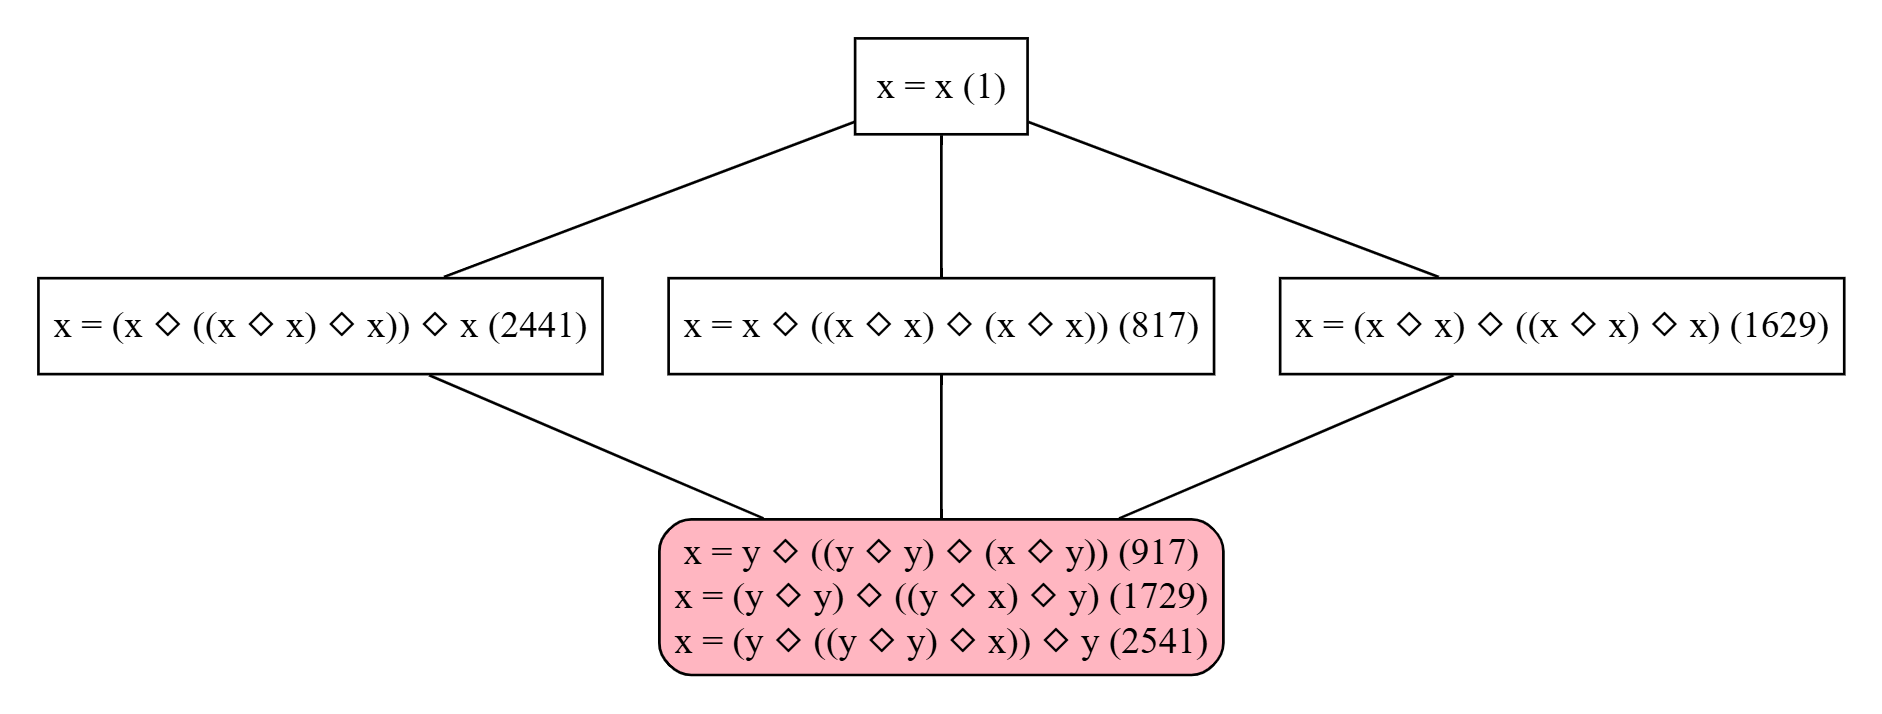
\includegraphics[width=0.4\textwidth]{ramanujan-finite.png}
    \caption{A Hasse diagram of all the equational laws implied by \eqref{eq1729}, both for unrestricted magmas (left) and finite magmas (right). Note the slightly larger number of implications in the latter.}
    \label{fig:1729}
\end{figure}

\begin{figure}
    \centering
    \resizebox{\textwidth}{!}{%
      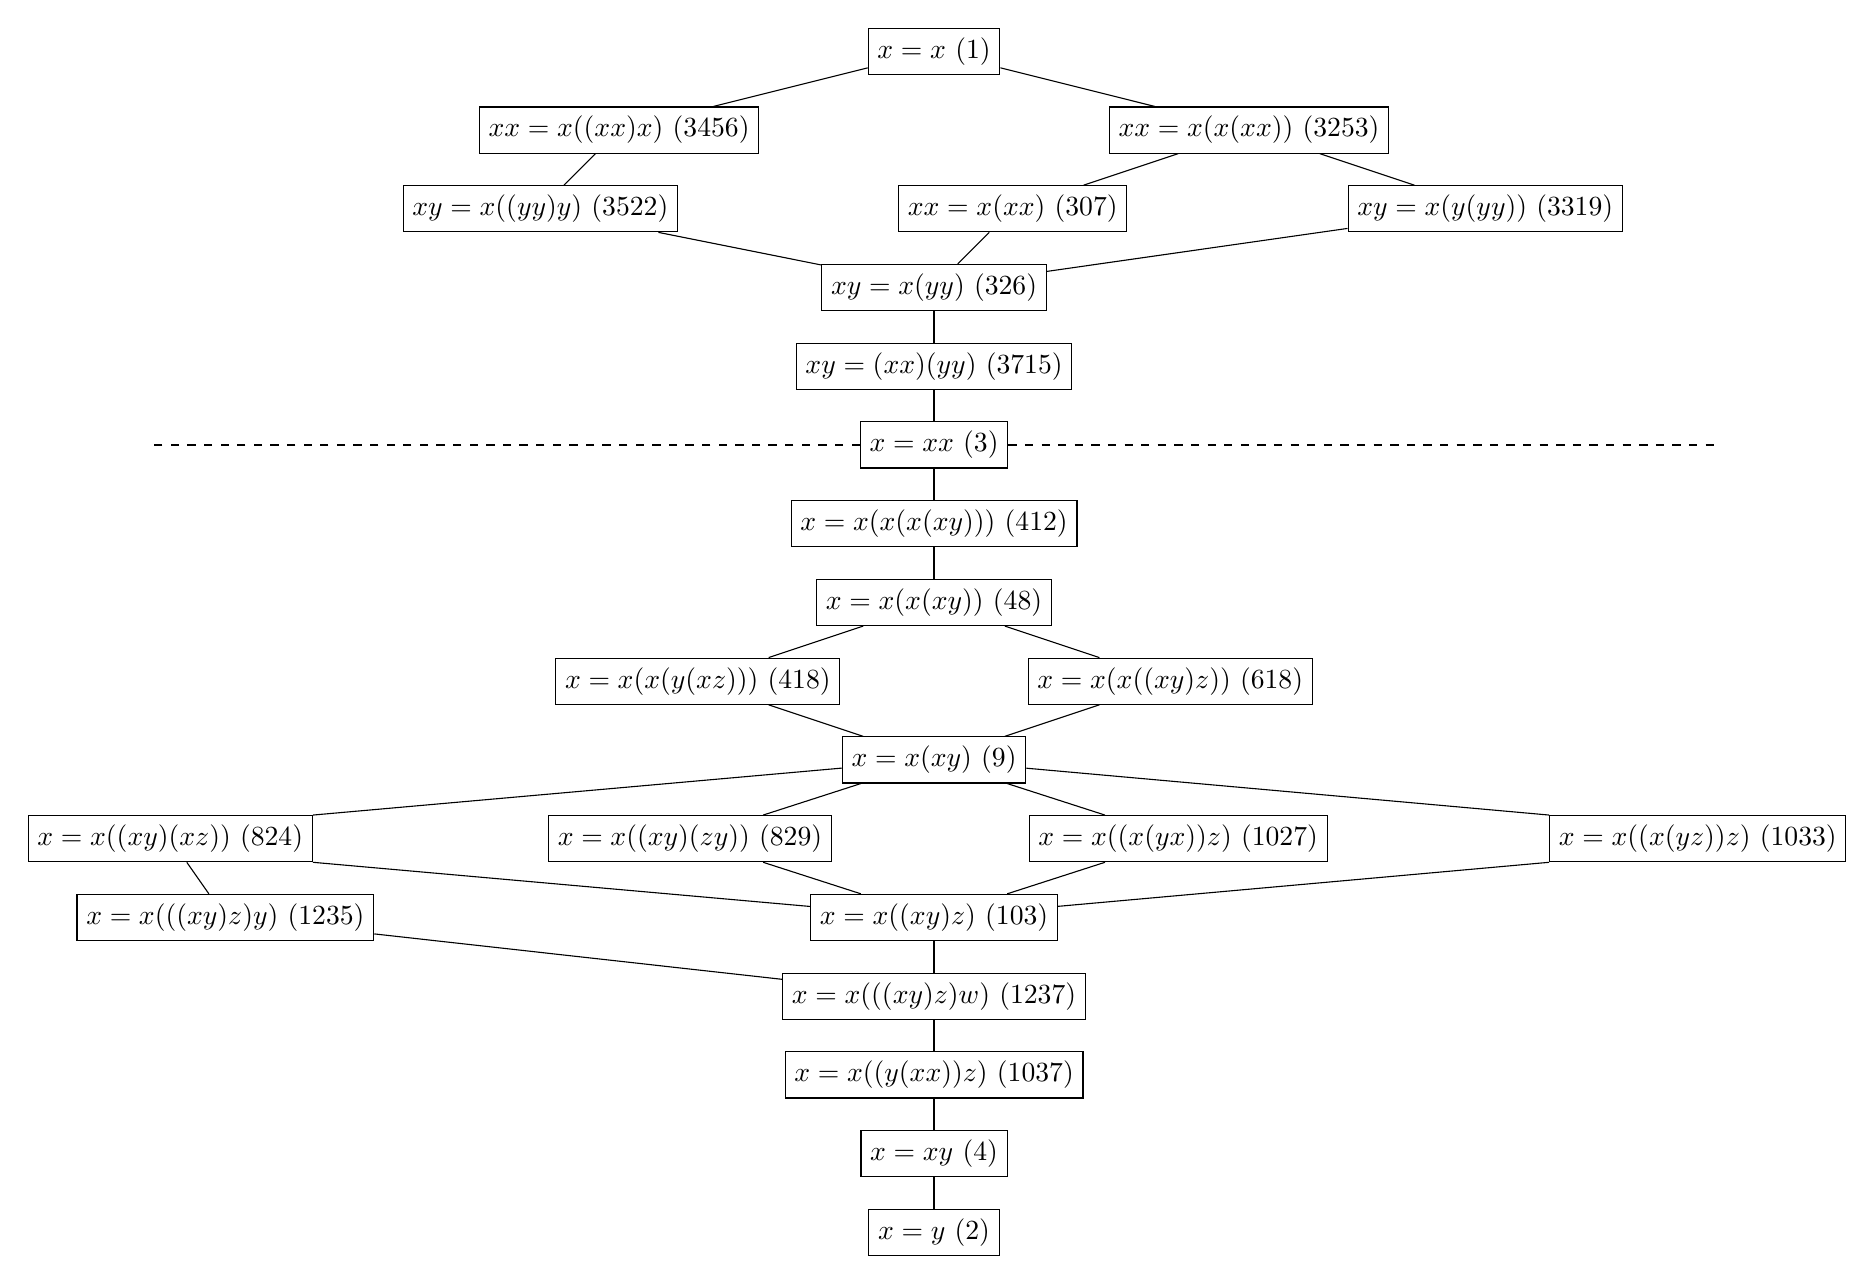
\begin{tikzpicture}
        \node(1)[draw] at (0,15) {$x = x$ (1)};
        \node(3253)[draw] at (4,14) {$x \op x = x \op (x \op (x \op x))$ (3253)};
        \node(3456)[draw] at (-4,14) {$x \op x = x \op ((x \op x) \op x)$ (3456)};
        \node(3319)[draw] at (7,13) {$x \op y = x \op (y \op (y \op y))$ (3319)};
        \node(307)[draw] at (1,13) {$x \op x = x \op (x \op x)$ (307)};
        \node(3522)[draw] at (-5,13) {$x \op y = x \op ((y \op y) \op y)$ (3522)};
        \node(326)[draw] at (0,12) {$x \op y = x \op (y \op y)$ (326)};
        \node(3715)[draw] at (0,11) {$x \op y = (x \op x) \op (y \op y)$ (3715)};
        \node(3)[draw] at (0,10) {$x = x \op x$ (3)};
        \draw[dashed](3)--(-10,10);
        \draw[dashed](3)--(10,10);
        \node(412)[draw] at (0,9) {$x = x \op (x \op (x \op (x \op y)))$ (412)};
        \node(48)[draw] at (0,8) {$x = x \op (x \op (x \op y))$ (48)};
        \node(618)[draw] at (3,7) {$x = x \op (x \op ((x \op y) \op z))$ (618)};
        \node(418)[draw] at (-3,7) {$x = x \op (x \op (y \op (x \op z)))$ (418)};
        \node(9)[draw] at (0,6) {$x = x \op (x \op y)$ (9)};
        \node(824)[draw] at (-9.7,5) {$x = x \op ((x \op y) \op (x \op z))$ (824)};
        \node(829)[draw] at (-3.1,5) {$x = x \op ((x \op y) \op (z \op y))$ (829)};
        \node(1027)[draw] at (3.1,5) {$x = x \op ((x \op (y \op x)) \op z)$ (1027)};
        \node(1033)[draw] at (9.7,5) {$x = x \op ((x \op (y \op z)) \op z)$ (1033)};
        \node(103)[draw] at (0,4) {$x = x \op ((x \op y) \op z)$ (103)};
        \node(1235)[draw] at (-9,4) {$x = x \op (((x \op y) \op z) \op y)$ (1235)};
        \node(1237)[draw] at (0,3) {$x = x \op (((x \op y) \op z) \op w)$ (1237)};
        \node(1037)[draw] at (0,2) {$x = x \op ((y \op (x \op x)) \op z)$ (1037)};
        \node(4)[draw] at (0,1) {$x = x \op y$ (4)};
        \node(2)[draw] at (0,0) {$x = y$ (2)};
        \draw(2)--(4);
        \draw(4)--(1037);
        \draw(1037)--(1237);
        \draw(1237)--(1235);
        \draw(1235)--(824);
        \draw(1237)--(103);
        \draw(103)--(1027);
        \draw(103)--(1033.south west);
        \draw(103)--(824.south east);
        \draw(103)--(829);
        \draw(1027)--(9);
        \draw(1033.north west)--(9);
        \draw(829)--(9);
        \draw(824.north east)--(9);
        \draw(9)--(418);
        \draw(9)--(618);
        \draw(418)--(48);
        \draw(618)--(48);
        \draw(48)--(412);
        \draw(412)--(3);
        \draw(3)--(3715);
        \draw(3715)--(326);
        \draw(326)--(3522);
        \draw(3522)--(3456);
        \draw(3456)--(1);
        \draw(326)--(307);
        \draw(307)--(3253);
        \draw(3253)--(1);
        \draw(326)--(3319);
        \draw(3319)--(3253);
      \end{tikzpicture}%
    }
    \caption{Longest chains of implications (length $15$) between inequivalent laws in the implication graph.  The parts above/below law 3 can be independently dualized. }
    \label{fig:longchain}
\end{figure}

Of the $\num{22033636}$ possible implications $E \vdash E'$, $8178279$ (or $37.12\%$) would end up being true; for an additional set of either $820$ or $822$ pairs $E,E'$, the weaker implication $E \vdashfin E'$ also held. To establish such positive implications $E \vdash E'$ or $E \vdashfin E'$, the main techniques used were as follows:

\begin{itemize}
    \item A very small number of positive implications were established and \textbf{formalized by hand}, mostly through direct rewriting of the laws; but this approach would not scale to the full project.
    \item \textbf{Simple rewriting rules}, for instance based on the observation that any law of the form $\x \formaleq f(\y,\z,\dots)$ was necessarily equivalent to the trivial law \eqref{eq2}, could already reduce the size of potential equivalence classes by a significant fraction. We discuss this method in \Cref{rewrite-sec}.
    \item The preorder axioms for $\vdash$, as well as the ``duality'' symmetry of the preorder with respect to replacing a magma operation $x \op y$ with its opposite $x \op^{\mathrm{op}} y \coloneqq y \op x$, can be used to significantly cut down on the number of implications that need to be proven explicitly; ultimately, only $10657$ ($0.13\%$) of the positive implications needed a direct proof.
    \item To obtain additional implications for finite magmas, heavy reliance was made on the fact that for functions $f \colon M \to M$ on a finite set $M$, surjectivity was equivalent to injectivity.  Some more sophisticated variants of this idea can lead to additional implications; see \Cref{finite-sec}.
    \item \textbf{Automated Theorem Provers} (ATP) could be deployed at extremely fast speeds to establish a complete generating set of positive implications; see \Cref{automated-sec}.
\end{itemize}

More challenging were the $\num{13855357}$ ($62.88\%$) implications that were false, $E \nvdash E'$, and particularly the slightly smaller set of $\num{13854535}$ or $\num{13854537}$ implications that were false even for finite magmas, $E \nvdashfin E'$. Here, the range of techniques needed to refute such implications were quite varied, and may be of independent interest:
\begin{itemize}
        \item \textbf{Syntactic methods}, such as observing a ``matching invariant'' of the law $E$ that was not shared by the law $E'$, could be used to obtain some refutations.  For instance, if both sides of $E$ had the same order, but both sides of $E'$ did not, this could be used to syntactically refute $E \vdash E'$.  Similarly, if the law $E$ was confluent, enjoyed a complete rewriting system, or otherwise permitted some understanding of the free magma associated to that law, one could decide the assertions $E \vdash E'$ for all possible laws $E'$, or at least a significant fraction of such laws.  We discuss these methods, and the extent to which they can be automated, in \Cref{syntactic-sec}.
        \item \textbf{Small finite magmas}, which can be described explicitly by multiplication tables, could be tested by brute force computations to provide a large number of finite counterexamples to implications, or by ATP-assisted methods. See \Cref{finite-sec}.
        \item \textbf{Linear models}, in which the magma operation took the form $x \op y = ax + by$ for some (commuting or noncommuting) coefficients $a,b$, allowed for another large class of counterexamples to implications, which could be automatically scanned for either by brute force or by Grobner basis type calculations; many of these examples could also be made finite. See \Cref{linear-sec}.
        \item \textbf{Translation invariant models}, in which the magma operation took the form $x \op y = x + f(y-x)$ on an additive group, or $x \op y = x f(x^{-1} y)$ on a noncommutative group, reduce matters to analyzing certain functional equations; see \Cref{translation-sec}.
        \item \textbf{Greedy methods}, in which either the multiplication table $(x,y) \mapsto x \op y$ or the function $f$ determining a translation-invariant model are iteratively constructed by a greedy algorithm subject to a well-chosen ruleset, were effective in resolving many implications not easily disposed of by preceding methods. See \Cref{greedy-sec}.
        \item Starting with a simple base magma $\Magma$ obeying both $E$ and $E'$, and either \textbf{enlarging} it to a larger magma $\Magma'$ containing $\Magma$ as a submagma, \textbf{extending} it to a magma $\MagmaN$ with a projection homomorphism $\pi: \MagmaN \to \Magma$, or \emph{modifying the multiplication table} on a small number of values, also proved effective when combined with greedy methods or with a ``\textbf{magma cohomology}'' construction. See \Cref{modify-base}.
        \item To each equation $E$ one can associate a ``\textbf{twisting semigroup}'' $S_E$.  If $S_E$ is larger than $S_{E'}$, then this can often be used to disprove the implication $E \vdash E'$; see \Cref{twisting-sec}.
        \item Some \textbf{ad hoc models} based on existing mathematical objects, such as infinite trees, rings of polynomials, or ``Kisielewicz models'' utilizing the prime factorization of the natural numbers, could also handle some otherwise difficult cases.  In some cases, the magma law induced some relevant and familiar structures, such as a directed graph or a partial order, which also helped guide counterexample constructions. We will not detail these diverse examples here, but refer the reader to the ETP blueprint for more discussion.
        \item \textbf{Automated theorem provers} were helpful in identifying which simplifying axioms could be added to the magma without jeopardizing the ability to refute the desired implication $E \vdash E'$ or $E \vdashfin E'$.
\end{itemize}

While the vast majority of negative implications could be quickly resolved by one of the above techniques, either with human input or in a completely automated fashion, there were perhaps two dozen such negative results that required quite delicate and \emph{sui generis} constructions.  The hardest such implication, $\Eq{1729} \nvdash \Eq{817}$, took several months to establish and then formalize (using a combination of many of the above constructions), with the final proof in \emph{Lean} requiring just over $\num{4000}$ dedicated lines of code from multiple contributors.

In the course of completing the implication graph, some interesting new algebraic structures were discovered.  One such example concerns the magmas obeying \eqref{eq1485}, which we refer to as \emph{weak central groupoids} as they contain the central groupoids (obeying \eqref{eq168}) as a subclass.  In \cite{knuth} it was observed that all finite central groupoids have order equal to a perfect square $n^2$; empirically, we have found that finite weak central groupoids always have order $n^2$ or $2n^2$, although we have no rigorous proof of this claim; they also have a graph-theoretic interpretation analogous to the interpretation of central groupoids as digraphs with the unique path property.  For these and other observations we refer the reader to \href{https://teorth.github.io/equational_theories/blueprint/weak-central-groupoids-chapter.html}{the blueprint of the ETP}.

The objective of using the data from the ETP to establish well-calibrated benchmarks to evaluate ATPs remains an interesting open problem; the participants of this project did not have the required expertise to develop and test such benchmarks to the standards expected in the area.  However, in \Cref{automated-sec} we present a more informal ``field report'' of our experiences using ATPs in the project, in the hope that this will provide some useful guidance to other researchers seeking to incorporate ATPs into their own research.

\begin{figure}
\centering
\begin{tikzpicture}[
    >=Latex,
    node distance=1.1cm,
    every node/.style={draw, rectangle, align=center},
    label/.style={font=\bfseries}
  ]

  %% Column labels
  \node[label] (ghlabel)   at (0,2) {GitHub};
  \node[label] (zuliplabel) at (7,2) {Lean Zulip};

  %% GitHub nodes
  \node (blueprint)   {Blueprint};
  \node (formal)     [below=of blueprint] {Lean formalization};
  \node (viz)        [below=of formal]    {Visualization tools};

  %% Lean Zulip nodes
  \node (hproofs)    [right=of blueprint]       {Human-gen. proofs};
  \node (cproofs)    [right=3cm of formal]         {Computer-gen. proofs};
  \node (hdisc)      [right=of viz]         {Human discussion};

  %% External ATP box
  \node (atp)        [right=of cproofs]         {ATPs, other\\external tools};

  %% Grouping boxes
  % GitHub container
  \node[draw,dotted,inner sep=8pt,fit=(blueprint)(formal)(viz), label=above:GitHub]
    (ghbox) {};
  % Lean Zulip container
  \node[draw,dotted,inner sep=8pt,fit=(hproofs)(cproofs)(hdisc), label=above:Lean Zulip]
    (zulipbox) {};

  %% Arrows
  \draw[human,->] (blueprint)  -- (formal);
  \draw[auto,->] (formal)     -- (viz);
  \draw[human,->] (viz)        -- (hdisc);
  \draw[human,->] (hdisc)      -- (atp);
  \draw[auto,->] (atp)        -- (cproofs);
  \draw[human,->] (cproofs)    -- (hproofs);
  \draw[semi,->] (cproofs)    -- (formal);
  \draw[human,<->] (hproofs)   -- (hdisc);
  \draw[human,->] (hproofs)  -- (blueprint);
  \draw[human,->] (hproofs)  -- (formal);

\end{tikzpicture}
\caption{Some of the main dynamics in which proofs were generated, discussed within the Lean Zulip channel and then formalized in the Github repository.  Boldface arrows indicate human activities, such as proposing an automated attack on outstanding implications, converting a computer-generated proof into a human-readable format, formalizing a human readable proof directly, or first creating a more precise blueprint for other collaborators to work on.  Dashed arrows indicate fully automated processes, while the partly dashed line indicated a semi-automated process requiring human supervision. }
\label{fig:flow}
\end{figure}

\subsection{Further directions}

While the primary objective of the ETP was being completed, some additional related results were generated as spinoffs.  Specifically:
\begin{itemize}
\item In the blueprint on the ETP web site, we report some partial progress on classifying which of the $57882$ distinct laws of order $5$ are equivalent to the singleton law \eqref{eq2}, either with or without the requirement that the magma be finite.
\item In \Cref{higman-neumann} we report on classifying the laws of order $8$ that are equivalent to the Higman-Neumann law \eqref{eq42323216}.
\item In \Cref{ml-sec} we report on preliminary experiments on using machine learning to determine to what extent the implication graph can be predicted by a neural network.
\end{itemize}

\chapter{Selected laws}\label{subgraph-eq}

In this project we study the 4694 laws (up to symmetry and relabeling) of total order at most $4$.

Selected laws of interest are listed below, as well as in \href{https://github.com/teorth/equational_theories/blob/main/equational_theories/Equations.lean}{this file}.

\begin{definition}[Equation 1]\label{eq1}\lean{Equation1}\leanok\uses{magma-def}  Equation 1 is the law $0 \formaleq 0$ (or the equation $x=x$).
\end{definition}

This is the trivial law, satisfied by all magmas. It is self-dual.


\begin{definition}[Equation 2]\label{eq2}\lean{Equation2}\leanok\uses{magma-def}  Equation 2 is the law $0 \formaleq 1$ (or the equation $x=y$).
\end{definition}

This is the singleton law, satisfied only by the empty and singleton magmas.  It is self-dual.

\begin{definition}[Equation 3]\label{eq3}\lean{Equation3}\leanok\uses{magma-def}  Equation 3 is the law $0 \formaleq 0 \op 0$ (or the equation $x = x \op x$).
\end{definition}

This is the idempotence law.  It is self-dual.

\begin{definition}[Equation 4]\label{eq4}\lean{Equation4}\leanok\uses{magma-def}  Equation 4 is the law $0 \formaleq 0 \op 1$ (or the equation $x = x \op y$).
\end{definition}

This is the left absorption law.

\begin{definition}[Equation 5]\label{eq5}\lean{Equation5}\leanok\uses{magma-def}  Equation 5 is the law $0 \formaleq 1 \op 0$ (or the equation $x = y \op x$).
\end{definition}

This is the right absorption law (the dual of Definition \ref{eq4}).

\begin{definition}[Equation 6]\label{eq6}\lean{Equation6}\leanok\uses{magma-def}  Equation 6 is the law $0 \formaleq 1 \op 1$ (or the equation $x = y \op y$).
\end{definition}

This law is equivalent to the singleton law.

\begin{definition}[Equation 7]\label{eq7}\lean{Equation7}\leanok\uses{magma-def}  Equation 7 is the law $0 \formaleq 1 \op 2$ (or the equation $x = y \op z$).
\end{definition}

This law is equivalent to the singleton law.

\begin{definition}[Equation 8]\label{eq8}\lean{Equation8}\leanok\uses{magma-def}  Equation 8 is the law $0 \formaleq 0 \op (0 \op 0)$ (or the equation $x = x \op (x \op x)$).
\end{definition}

\begin{definition}[Equation 14]\label{eq14}\lean{Equation14}\leanok\uses{magma-def}  Equation 14 is the law $0 \formaleq  1 \op (0 \op 1)$ (or the equation $x = y \op (x \op y))$.
\end{definition}

Appears in Problem A1 from Putnam 2001.

\begin{definition}[Equation 16]\label{eq16}\lean{Equation16}\leanok\uses{magma-def}  Equation 16 is the law $0 \formaleq  1 \op (1 \op 0)$ (or the equation $x = y \op (y \op x))$.
\end{definition}

\begin{definition}[Equation 23]\label{eq23}\lean{Equation23}\leanok\uses{magma-def}  Equation 23 is the law $0 \formaleq  (0 \op 0) \op 0$ (or the equation $x = (x \op x) \op x$).
\end{definition}

This is the dual of Definition \ref{eq8}.

\begin{definition}[Equation 29]\label{eq29}\lean{Equation29}\leanok\uses{magma-def}  Equation 29 is the law $0 \formaleq  (1 \op 0) \op 1$ (or the equation $x = (y \op x) \op y)$.
\end{definition}

Appears in Problem A1 from Putnam 2001.  Dual to Definition \ref{eq14}.

\begin{definition}[Equation 38]\label{eq38}\lean{Equation38}\leanok\uses{magma-def}  Equation 38 is the law $0 \op 0  \formaleq  0 \op 1$ (or the equation $x \op x = x \op y$).
\end{definition}

This law asserts that the magma operation is independent of the second argument.

\begin{definition}[Equation 39]\label{eq39}\lean{Equation39}\leanok\uses{magma-def}  Equation 39 is the law $0 \op 0  \formaleq  1 \op 0$ (or the equation $x \op x = y \op x$).
\end{definition}

This law asserts that the magma operation is independent of the first argument (the dual of Definition \ref{eq38}).

\begin{definition}[Equation 40]\label{eq40}\lean{Equation40}\leanok\uses{magma-def}  Equation 40 is the law $0 \op 0  \formaleq  1 \op 1$ (or the equation $x \op x = y \op y$).
\end{definition}

This law asserts that all squares are constant. It is self-dual.

\begin{definition}[Equation 41]\label{eq41}\lean{Equation41}\leanok\uses{magma-def}  Equation 41 is the law $0 \op 0  \formaleq  1 \op 2$ (or the equation $x \op x = y \op z$).
\end{definition}

This law is equivalent to the constant law, Definition \ref{eq46}.

\begin{definition}[Equation 42]\label{eq42}\lean{Equation42}\leanok\uses{magma-def}  Equation 42 is the law $0 \op 1  \formaleq  0 \op 2$ (or the equation $x \op y = x \op z$).
\end{definition}

Equivalent to Definition \ref{eq38}.

\begin{definition}[Equation 43]\label{eq43}\lean{Equation43}\leanok\uses{magma-def}  Equation 43 is the law $0 \op 1  \formaleq  1 \op 0$ (or the equation $x \op y = y \op x$).
\end{definition}

The commutative law. It is self-dual.

\begin{definition}[Equation 45]\label{eq45}\lean{Equation45}\leanok\uses{magma-def}  Equation 45 is the law $0 \op 1  \formaleq  2 \op 1$ (or the equation $x \op y = z \op y$).
\end{definition}

This is the dual of Definition \ref{eq42}.

\begin{definition}[Equation 46]\label{eq46}\lean{Equation46}\leanok\uses{magma-def}  Equation 46 is the law $0 \op 1  \formaleq  2 \op 3$ (or the equation $x \op y = z \op w$).
\end{definition}

The constant law: all products are constant. It is self-dual.

\begin{definition}[Equation 168]\label{eq168}\lean{Equation168}\leanok\uses{magma-def}  Equation 168 is the law $0  \formaleq  (1 \op 0) \op (0 \op 2)$ (or the equation $x = (y \op x) \op (x \op z)$).
\end{definition}

The law of a central groupoid. It is self-dual.

\begin{definition}[Equation 381]\label{eq381}\lean{Equation381}\leanok\uses{magma-def}  Equation 381 is the law $0 \op 1  \formaleq  (0 \op 2) \op 1$ (or the equation $x \op y = (x \op z) \op y$).
\end{definition}

Appears in Putnam 1978, Problem A4, part (b).

\begin{definition}[Equation 387]\label{eq387}\lean{Equation387}\leanok\uses{magma-def}  Equation 387 is the law $0 \op 1  \formaleq  (1 \op 1) \op 0$ (or the equation $x \op y = (y \op y) \op x$).
\end{definition}

Introduced in \href{https://mathoverflow.net/a/450905/766}{MathOverflow}.

\begin{definition}[Equation 953]\label{eq953}\lean{Equation953}\leanok\uses{magma-def}  Equation 953 is the law $0 = 1 \op ((2 \op 0) \op (2 \op 2))$ (or the equation $x = y \op ((z \op x) \op (z \op z))$).
\end{definition}

\begin{definition}[Equation 1571]\label{eq1571}\lean{Equation1571}\leanok\uses{magma-def}  Equation 1571 is the law $0 \formaleq  (1 \op 2) \op (1 \op (0 \op 2))$ (or the equation $x = (y \op z) \op (y \op (x \op z))$).
\end{definition}

Introduced in \cite{mendelsohn-padmanabhan}.

\begin{definition}[Equation 1689]\label{eq1689}\lean{Equation1689}\leanok\uses{magma-def}  Equation 1689 is the law $0 \formaleq  (1 \op 0) \op ((0 \op 2) \op 2)$ (or the equation $x = (y \op x) \op ((x \op z) \op z)$).
\end{definition}

Mentioned in \cite{Kisielewicz2}.

\begin{definition}[Equation 2662]\label{eq2662}\lean{Equation2662}\leanok\uses{magma-def}  Equation 2662 is the law $0 \formaleq  ((0 \op 1) \op (0 \op 1)) \op 0$ (or the equation $x = ((x \op y) \op (x \op y)) \op x$).
\end{definition}

Appears in \cite{mendelsohn-padmanabhan}.

\begin{definition}[Equation 3722]\label{eq3722}\lean{Equation3722}\leanok\uses{magma-def}  Equation 3722 is the law $0 \op 1  \formaleq  (0 \op 1) \op (0 \op 1)$ (or the equation $x \op y = (x \op y) \op (x \op y)$).
\end{definition}

Appears in Putnam 1978, Problem A4, part (a).  It is self-dual.

\begin{definition}[Equation 3744]\label{eq3744}\lean{Equation3744}\leanok\uses{magma-def}  Equation 3744 is the law $0 \op 1  \formaleq  (0 \op 2) \op (3 \op 1)$ (or the equation $x \op y = (x \op z) \op (w \op y)$).
\end{definition}

This law is called a ``bypass operation'' in Putnam 1978, Problem A4. It is self-dual.

\begin{definition}[Equation 4512]\label{eq4512}\lean{Equation4512}\leanok\uses{magma-def}  Equation 4512 is the law $0 \op (1 \op 2)  \formaleq  (0 \op 1) \op 2$ (or the equation $x \op (y \op z) = (x \op y) \op z$).
\end{definition}

The associative law. It is self-dual.

\begin{definition}[Equation 4513]\label{eq4513}\lean{Equation4513}\leanok\uses{magma-def}  Equation 4513 is the law $0 \op (1 \op 2)  \formaleq  (0 \op 1) \op 3$ (or the equation $x \op (y \op z) = (x \op y) \op w$).
\end{definition}

\begin{definition}[Equation 4522]\label{eq4522}\lean{Equation4522}\leanok\uses{magma-def}  Equation 4522 is the law $0 \op (1 \op 2)  \formaleq  (0 \op 3) \op 4$ (or the equation $x \op (y \op z) = (x \op w) \op u$).
\end{definition}

Dual to Definition \ref{eq4579}.

\begin{definition}[Equation 4564]\label{eq4564}\lean{Equation4564}\leanok\uses{magma-def}  Equation 4564 is the law $0 \op (1 \op 2)  \formaleq  (3 \op 1) \op 2$ (or the equation $x \op (y \op z) = (w \op y) \op z$).
\end{definition}

Dual to Definition \ref{eq4513}.

\begin{definition}[Equation 4579]\label{eq4579}\lean{Equation4579}\leanok\uses{magma-def}  Equation 4579 is the law $0 \op (1 \op 2)  \formaleq  (3 \op 4) \op 2$ (or the equation $x \op (y \op z) = (w \op u) \op z$).
\end{definition}

Dual to Definition \ref{eq4522}.

\begin{definition}[Equation 4582]\label{eq4582}\lean{Equation4582}\leanok\uses{magma-def}  Equation 4582 is the law $0 \op (1 \op 2)  \formaleq  (3 \op 4) \op 5$ (or the equation $x \op (y \op z) = (w \op u) \op v$).
\end{definition}

This law asserts that all triple constants (regardless of bracketing) are constant.

We also note some selected laws of order more than $5$.

\begin{definition}[Equation 5105]
  \label{eq5105}\uses{magma-def}
  Equation 5105 is the law $0  \formaleq 1 \circ (1 \circ (1 \circ (0 \circ (2 \circ 1))))$ (or the equation $x = y \circ (y \circ (y \circ (x \circ (z \circ y))))$).
\end{definition}

This law of order $5$ was mentioned in \cite{Kisielewicz2}.

\begin{definition}[Equation 28393]
  \label{eq28393}\uses{magma-def}
  Equation 28393 is the law $0  \formaleq  (((1 \circ 1) \circ 1) \circ 0) \circ (1 \circ 2)$ (or the equation $x = (((y \circ y) \circ y) \circ x) \circ (y \circ z)$).
\end{definition}

This law of order $5$ was introduced by Kisielewicz \cite{Kisielewicz}.

\begin{definition}[Equation 374794]
  \lean{Equation374794}\leanok
  \label{eq374794}\uses{magma-def}
  Equation 374794 is the law $0  \formaleq  (((1 \circ 1) \circ 1) \circ 0) \circ ((1 \circ 1) \circ 2)$ (or the equation $x = (((y \circ y) \circ y) \circ x) \circ ((y \circ y) \circ z)$).
\end{definition}

This law of order $6$ was introduced by Kisielewicz \cite{Kisielewicz}.

The singleton or empty magma obeys all equational laws.  One can ask whether an equational law admits nontrivial finite or infinite models.  An \emph{Austin law} is a law which admits infinite models, but no nontrivial finite models.  Austin \cite{austin} established the first such law, namely the order $9$ law
$$ (((1 \circ 1) \circ 1) \circ 0) \circ (((1 \circ 1) \circ ((1 \circ 1) \circ 1)) \circ 2) \formaleq 0.$$
A shorter Austin law of order $6$ was established in \cite{Kisielewicz}:

\begin{theorem}[Kisielewicz's first Austin law]
  \lean{InfModel.Finite.Equation374794_implies_Equation2,InfModel.Equation374794_not_implies_Equation2}\leanok
  \label{kis-thm}\uses{eq374794,eq2}
  Definition \ref{eq374794} is an Austin law.
\end{theorem}

\begin{proof} \leanok Suppose for contradiction that we have a non-trivial model of Definition \ref{eq374794}. Write $y^2 := y \circ y$ and $y^3 := y^2 \circ y$. For any $y,z$, introduce the functions $f_y: x \mapsto y^3 \circ x$ and $g_{yz}: x \mapsto x \circ (y^2 \circ z)$.  Definition \ref{eq374794} says that $g_{yz}$ is a left-inverse of $f_y$, hence by finiteness these are inverses and $g_{yz}$ is independent of $z$. In particular
$$ f(y^3) = g_{yy}(y^3) = g_{yz}(y^3) = f(y^2 \circ z)$$
and hence $y^2 \circ z$ is independent of $z$.  Thus
$$ f_y(x) = (y^2 \circ y) \circ x = (y^2 \circ y^2) \circ x$$
is independent of $x$.  As $f_y$ is invertible, this forces the magma to be trivial, a contradiction.

To construct an infinite magma, take the positive integers $\Z^+$ with the operation $x \circ y$ defined as
\begin{itemize}
  \item $2^x$ if $y=x$;
  \item $3^y$ if $x = 1 \neq y$;
  \item $\min(j,1)$ if $x=3^j$ and $y \neq x$; and
  \item $1$ otherwise.
\end{itemize}
Then $y^2 = 2^y$, $y^3 = 1$, and $y^2 \circ z$ a power of two for all $y, z$, and $(1 \circ x) \circ w = x$ for all $x$ whenever $w$ is a power of two, so Definition \ref{eq374794} is satisfied.
\end{proof}

An even shorter law (order $5$) was obtained by the same author in a followup paper \cite{Kisielewicz2}:

\begin{theorem}[Kisielewicz theoremII]\label{kis-thm2}\uses{eq2} Definition \ref{eq28393} is an Austin law.
\end{theorem}

\begin{proof} Using the $y^2$ and $y^3$ notation as before, the law reads
\begin{equation}\label{kis2-law}
   x = (y^3 \circ x) \circ (y \circ z).
  \end{equation}
In particular, for any $y$, the map $T_y \colon x \mapsto y^3 \circ x$ is injective, hence bijective in a finite model $G$.  In particular we can find a function $f : G \to G$ such that $T_y f(y) = y^3$ for all $y$  Applying \eqref{kis2-law} with $x = f(y)$, we conclude
$$ T_y(y \circ z) = y^3 \circ (y \circ z) = f(y) $$
and thus $y \circ z$ is independent of $z$ by injectivity of $T_y$.  Thus, the left-hand side of \eqref{kis2-law} does not depend on $x$, and so the model is trivial.  This shows there are no non-trivial finite models.

To establish an infinite model, use $\N$ with $x \circ y$ defined by requiring
$$ y \circ y = 2^y; \quad 2^y \circ y = 3^y$$
and
$$ 3^y \circ x = 3^y 5^x$$
for $x \neq 3^y$, and
$$ (3^y 5^x) \circ z = x$$
for $z \neq 3^y 5^x$.  Finally set
$$ 2^{3^y} \circ z = 3^y$$
for $z \neq 3^y, 2^{3^y}$.  All other assignments of $\circ$ may be made arbitrarily. It is then a routine matter to establish \eqref{kis2-law}.
\end{proof}

In that paper a computer search was also used to show that no law of order four or less is an Austin law.

An open question is whether Definition \ref{eq5105} is an Austin law.  We have the following partial result from \cite{Kisielewicz2}:

\begin{theorem}[Equation 5105 has no non-trivial finite models]\lean{InfModel.Finite.Equation5105_implies_Equation2}\leanok\label{5105-nontrivial}\uses{eq5105} Definition \ref{eq5105} has no non-trivial finite models.
\end{theorem}

\begin{proof} \leanok From Definition \ref{eq5105} we see that the map $w \mapsto y \circ w$ is onto, hence injective in a finite model.  Using this injectivity four times in Definition \ref{eq5105}, we see that $z \circ y$ does not depend on $z$, hence the expression
$x \circ (z \circ y)$ does not depend on $x$.  By Definition \ref{eq5105} again, this means that $x$ does not depend on $x$, which is absurd in a non-trivial model.
\end{proof}

\chapter{General implications}\label{generla-implications-chapter}
We will be interested in seeing which laws imply which other laws, in the sense that magmas obeying the former law automatically obey the latter. We will also be interested in \emph{anti-implications} showing that one law does \emph{not} imply another, by producing examples of magmas that obey the former law but not the latter. Here is a formal definition.

\begin{definition}[Implication]\label{impl}\uses{models-def}
  A law $E$ is said to \emph{imply} another law $E'$ if $\{E\} \models E'$, or equivalently:
  $$ G \models w  \formaleq  w' \implies G \models w''  \formaleq  w''' \hbox{ for all magmas } G$$
  Two laws are said to be \emph{equivalent} if they imply each other.
\end{definition}

\begin{lemma}[Pre-order]\leanok\label{pre-order}\uses{impl}
  If we define $E \leq E'$ if $E$ implies $E'$, then this is a pre-order on the set of laws, and equivalence is an equivalence relation.
\end{lemma}

Note that we view the stronger law as less than or equal to the weaker law. This is because the class of magmas that obey the stronger law is a subset of the class of magmas that obey the weaker law. It is also consistent with the conventions of Lean's Mathlib.

\begin{proof}\leanok
  Trivial.
\end{proof}

Implications between the laws from \Cref{subgraph-eq} are depicted in \Cref{fig:implications}.

\begin{figure}
  \centering
  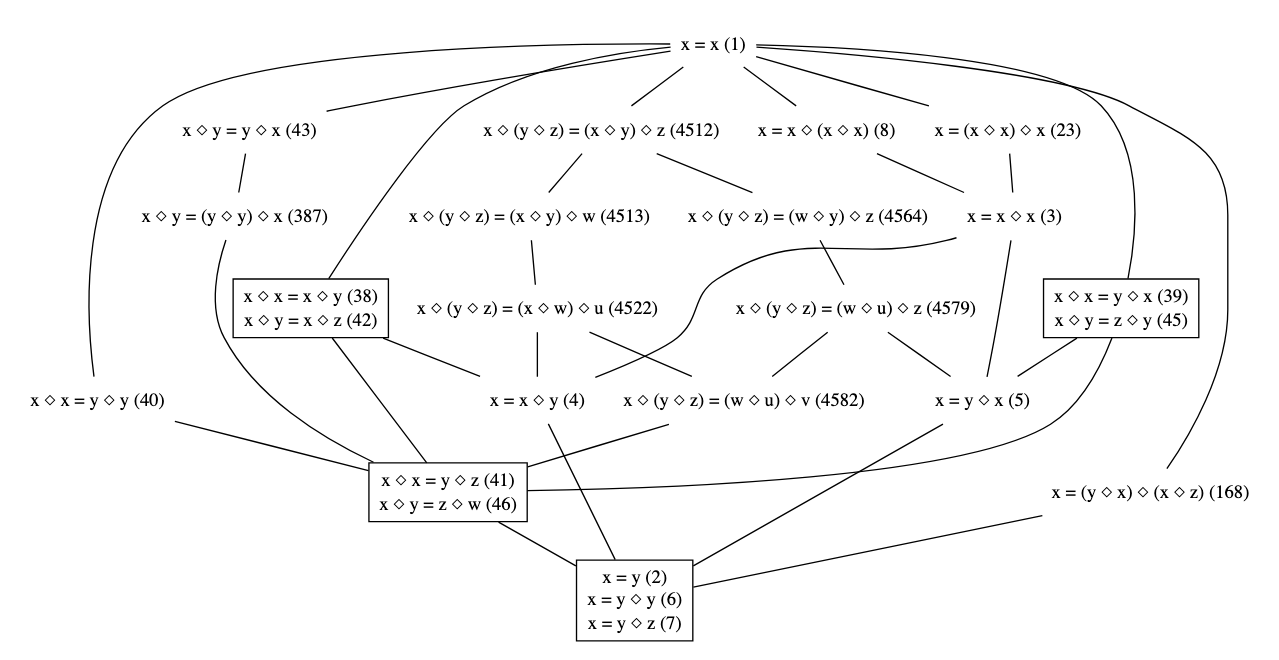
\includegraphics[width=1\linewidth]{../../images/subgraph.png}
  \caption{Implications between the above equations, displayed as a Hasse diagram.}
  \label{fig:implications}
\end{figure}

\begin{lemma}[Maximal element]\label{maximal}\uses{pre-order}\lean{Law.MagmaLaw.Equation1_maximal}\leanok
  The law $0  \formaleq  0$ is the maximal element in this pre-order.
\end{lemma}

\begin{proof}
  Trivial.
\end{proof}

\begin{lemma}[Minimal element]\label{minimal}\uses{pre-order}\lean{Law.MagmaLaw.Equation2_minimal}\leanok
  The law $0  \formaleq  1$ is the minimal element in this pre-order.
\end{lemma}

\begin{proof}
  Trivial.
\end{proof}

Every magma $G$ has a \emph{reversal} $G^{\mathrm{op}}$, formed by by replacing the magma operation $\op$ with its opposite $\op^{\mathrm{op}}:(x,y) \mapsto y \op x$. There is a natural isomorphism between these magmas, which induces an involution $w \mapsto w^{\mathrm{op}}$ on words $w \in M_X$. Every law $w  \formaleq  w'$ then has a \emph{dual} $w^{\mathrm{op}}  \formaleq  (w')^{\mathrm{op}}$.

For instance, the dual of the law $0 \op 1 = 0 \op 2$ is $1 \op 0 = 2 \op 0$, which after relabeling is $0 \op 1 = 2 \op 1$. A list of equations and their duals can be found \href{https://github.com/teorth/equational_theories/blob/main/data/dual_equations.md}{here}. Of the 4694 equations under consideration, 84 are self-dual, leaving 2305 pairs of dual equations.

The pre-ordering on laws has a duality symmetry:

\begin{lemma}[Duality of laws]\lean{Law.MagmaLaw.implies_iff_op}\leanok\label{duality}\uses{pre-order}
  The law $w  \formaleq  w'$ implies $w''  \formaleq  w'''$, if and only if $w^{\mathrm{op}}  \formaleq  (w')^{\mathrm{op}}$ implies $w''^{\mathrm{op}}  \formaleq  (w''')^{\mathrm{op}}$.
\end{lemma}

\begin{proof}
  This follows from the fact that a magma $G$ satisfies a law $w  \formaleq  w'$ if and only if $G^{\mathrm{op}}$ satisfies $w^{\mathrm{op}}  \formaleq  (w')^{\mathrm{op}}$.
\end{proof}

Some equational laws can be ``diagonalized'':

\begin{theorem}[Diagonalization]\label{diag}
  An equational law of the form
  \begin{equation}\label{prediag}
    F(x_1,\dots,x_n) = G(y_1,\dots,y_m),
  \end{equation}
  where $x_1,\dots,x_n$ and $y_1,\dots,y_m$ are distinct elements of the alphabet, implies the diagonalized law
  $$ F(x_1,\dots,x_n) = F(x'_1,\dots,x'_n).$$
  where $x'_1,\dots,x'_n$ are distinct from $x_1,\dots,x_n$
  In particular, if $G(y_1,\dots,y_m)$ can be viewed as a specialization of $F(x'_1,\dots,x'_n)$, then these two laws are equivalent.
\end{theorem}

\begin{proof}
  From two applications of \Cref{prediag} one has
  $$ F(x_1,\dots,x_n) = G(y_1,\dots,y_m)$$
  and
  $$ F(x'_1,\dots,x'_n) = G(y_1,\dots,y_m)$$
  whence the claim.
\end{proof}

Thus for instance, \Cref{eq7} is equivalent to \Cref{eq2}.

\begin{theorem}[Laws implied by the constant law]\label{constant-impl}\uses{impl,eq46}
  If $w, w'$ each have order at least one, then the law $w \formaleq w'$ is implied by the constant law (\Cref{eq46}). If exactly one of $w, w'$ has order zero, and the law $w \formaleq w'$ is not implied by the constant law.
\end{theorem}

\begin{proof}
  Routine.
\end{proof}

\begin{theorem}[Criterion for implication]\label{variable-impl}\uses{impl}\lean{Law.MagmaLaw.SameCount.derive}\leanok
  If $w \formaleq w'$ is such that every variable appears the same number of times in both $w$ and $w'$, and $w \formaleq w'$ implies another law $w'' \formaleq w'''$, then every variable appears the same number of times in both $w''$ and $w'''$.
\end{theorem}

\begin{proof}
  Consider the magma $\mathrm{MS}$ of multisets over an arbitrary set $A$ (which can be seen as finitely supported maps $A\rightarrow \N$), with the multiset addition law $+$. By hypothesis, this magma obeys $w \formaleq w'$, and hence $w'' \formaleq w'''$, giving the claim by comparing the orders of the elements of $A$ appearing in $w''$ and $w'''$ in this magma.
\end{proof}

\chapter{Completeness and compactness theorems}

We now generalize the implication concept from Definition \ref{impl}:

\begin{definition}[Semantic consequence]\label{semantic-def}\uses{law-def} Let $\Gamma$ be a collection of laws, and let $E$ be a law. We say that $E$ is a \emph{semantic consequence} of $\Gamma$, and write $\Gamma \models E$, if every magma that obeys every law in $\Gamma$, also obeys $E$.
\end{definition}

Definition \ref{impl} is basically the case where $\Gamma$ is a singleton.

\begin{definition}[Syntactic consequence]\label{syntactic-def}\uses{law-def, push} Let $\Gamma$ be a collection of laws, and let $E$ be a law. We say that $E$ is a \emph{syntactic consequence} of $\Gamma$, and write $\Gamma \vdash E$, if $E$ can be deduced from $\Gamma$ using the following rules of inference:
\begin{itemize}
\item If $E$ is an element of $\Gamma$, then $\Gamma \vdash E$.
\item For any word $w$, we have $\Gamma \vdash w \formaleq w$.
\item If $w,w'$ are words with $\Gamma \vdash w \formaleq w'$, then $\Gamma \vdash w' \formaleq w$.
\item If $w,w',w''$ are words with $\Gamma \vdash w \formaleq w'$ and $\Gamma \vdash w' \formaleq w''$, then $\Gamma \vdash w \formaleq w''$.
\item If $w,w'$ are words with $\Gamma \vdash w \formaleq w'$, and $\pi : \N \to \N$ is a function, then $\Gamma \vdash \pi_* w \formaleq \pi_* w'$.
\item If $w,w',v$ are words with $\Gamma \vdash w \formaleq w'$, then $\Gamma \vdash v \circ w \formaleq v \circ w'$ and $\Gamma \vdash w \circ v \formaleq w' \circ v$.
\end{itemize}
\end{definition}

\begin{theorem}[Completeness theorem]\label{completeness-thm}\uses{semantic-def,syntactic-def}  Let $\Gamma$ be a collection of laws, and let $E$ be a law.  Then $\Gamma \models E$ if and only if $\Gamma \vdash E$.
\end{theorem}

\begin{proof} (Sketch) The `only if' component is soundness, and follows from verifying that the rules of inference in Definition \ref{synctactic-def} holds for $\models$.  The `if` part is completeness, and is proven by constructing the magma of words, quotiented out by the relation $\Gamma \vdash w \formaleq w'$, which is easily seen to be an equivalence relation respecting the magma operation
\end{proof}

\begin{corollary}[Compactness theorem]\label{compactness-thm}\uses{semantic-def,syntactic-def}  Let $\Gamma$ be a collection of laws, and let $E$ be a law.  Then $\Gamma \models E$ if and only if there exists a finite subset $\Gamma'$ of $\Gamma$ such that $\Gamma' \models E$.
\end{corollary}

\begin{proof}\uses{completeness-thm} The claim is obvious for $\vdash$, and the claim then follows from Theorem \ref{completeness-thm}
\end{proof}

\chapter{Subgraph implications}

Interesting implications between the subgraph equations in Chapter \ref{subgraph-eq}. To reduce clutter, trivial or very easy implications will not be displayed here.

\begin{theorem}[387 implies 43]\label{387_implies_43}\uses{eq387,eq43}\lean{Subgraph.Equation387_implies_Equation43}\leanok  Definition \ref{eq387} implies Definition \ref{eq43}.
\end{theorem}

\begin{proof}\leanok (From \href{https://mathoverflow.net/a/450905/766}{MathOverflow}).
  By Definition \ref{eq387}, one has the law
\begin{equation}\label{387-again}
  (x \circ x) \circ y = y \circ x.
\end{equation}
Specializing to $y=x \circ x$, we conclude
$$(x \circ x) \circ (x \circ x) = (x \circ x) \circ x$$
and hence by another application of \eqref{eq387} we see that $x \circ x$ is idempotent:
\begin{equation}\label{idem}
  (x \circ x) \circ (x \circ x) = x \circ x.
\end{equation}
Now, replacing $x$ by $x \circ x$ in \eqref{387-again} and then using \eqref{idem} we see that
$$ (x \circ x) \circ y = y \circ (x \circ x)$$
so in particular $x \circ x$ commutes with $y \circ y$:
\begin{equation}\label{op-idem} (x \circ x) \circ (y \circ y) = (y \circ y) \circ (x \circ x).
\end{equation}
Also, from two applications of \eqref{387-again} one has
$$(x \circ x) \circ (y \circ y) = (y \circ y) \circ x = x \circ y.$$
Thus \eqref{op-idem} simplifies to $x \circ y = y \circ x$, which is Definition \ref{eq43}.
\end{proof}

\begin{theorem}[29 equivalent to 14]\label{29_equiv_14} \uses{eq29,eq14}\lean{Subgraph.Equation29_implies_Equation14}\leanok  Definition \ref{eq29} is equivalent to Definition \ref{eq14}.
\end{theorem}

This result was posed as Problem A1 from Putnam 2001.

\begin{proof}\leanok\uses{duality} By Lemma \ref{duality} it suffices to show that Definition \ref{eq29} implies Definition \ref{eq14}.  From Definition \ref{eq29} one has
  $$ x = ((x \circ y) \circ x) \circ (x \circ y)$$
  and also
  $$ y = (x \circ y) \circ x$$
  giving $x = y \circ (x \circ y)$, which is Definition \ref{eq14}.
\end{proof}

\begin{theorem}[14 implies 29]\label{14_implies_29} \uses{eq29,eq14}\lean{Subgraph.Equation14_implies_Equation29}\leanok  Definition \ref{eq14} implies Definition \ref{eq29}.
\end{theorem}

This result was posed as Problem A1 from Putnam 2001.

\begin{proof}\leanok
\end{proof}

% abbrev Equation381 (G: Type u) [Magma G] := ∀ x y z : G, x ∘ y = (x ∘ z) ∘ y
% abbrev Equation3744 (G : Type u) [Magma G] := ∀ x y z w : G, x ∘ y = (x ∘ z) ∘ (w ∘ y)

%theorem Equation3744_implies_Equation381 (G : Type*) [Magma G] (h: Equation3744 G) : Equation381 G :=
%fun x y z ↦ Eq.trans
%  (h x y z y) $ Eq.trans
%  (congrArg (fun a ↦ a ∘ (y ∘ y)) (h x z z x))
%  (Eq.symm $ h (x ∘ z) y (x ∘ z) y)
%/-- Putnam 1978, problem A4, part (a) -/

The following result was problem A4 on Putnam 1978.

\begin{theorem}[3744 implies 3722, 381]\label{3744_implies_3722_381}\uses{eq3744, eq3722, eq381} Definition \ref{eq3744} implies Definition \ref{eq3722} and Definition \ref{eq381}.
\end{theorem}

\begin{proof} By hypothesis, one has
$$x \circ y = (x \circ z) \circ (w \circ y)
  $$
for all $x,y,z,w$.  Various specializations of this give
\begin{align}
 x \circ y &= (x \circ z) \circ (y \circ y) \label{381-1} \\
 x \circ z &= (x \circ z) \circ (x \circ z) \label{381-2} \\
(x \circ z) \circ y &= ((x \circ z) \circ (x \circ z)) \circ (y \circ y) \label{381-3}.
\end{align}
The equation \eqref{381-2} gives Definition \ref{eq3722}, while \eqref{381-1}, \eqref{381-2}, \eqref{381-3} gives
$$ x \circ y = (x\circ z) \circ y$$
which is Definition \ref{eq381}.
\end{proof}

\begin{theorem}[1689 is equivalent to 2]\label{1689_equiv_2}\uses{eq1689, eq2} Definition \ref{eq1689} is equivalent to Definition \ref{eq2}.
\end{theorem}


\begin{proof}\leanok  The implication of Definition \ref{eq1689} from Definition \ref{eq2} is trivial.  The converse is a surprisingly long chain of implications; see pages 326--327 of \cite{Kisielewicz2}.

\end{proof}

\chapter{Selected magmas}\label{selected-magmas-chapter}

Each magma can be used to establish anti-implications: if $\Gamma$ is the set of all laws obeyed by a magma $G$, then we have $\neg E \leq E'$ whenever $E \in \Gamma$ and $E' \not \in \Gamma$.  Large numbers of implications can already be obtained from

\begin{itemize}
  \item All magmas of size at most $4$, up to isomorphism (of which \href{https://oeis.org/A001329}{there are $178\,985\,294$});
  \item All commutative magmas of size $5$, up to isomorphism (of which \href{https://oeis.org/A001425}{there are $254\,429\,900$});
  \item Cyclic groups $\Z/N\Z$ with $2 \leq N \leq 12$ and $x \op y = ax^2+bxy+cy^2+dx+ey$ for randomly chosen $a,b,c,d,e$.
  \item There are only \href{https://oeis.org/A057991}{$1411$ quasigroups of size $5$} (up to isomorphism), and Mace4 can generate all of them in under 20 seconds. A shell script to do this is available \href{https://github.com/zaklogician/equational_theories/tree/cancellative_magmas/scripts/cancellative_magmas}{here}. A magma is a quasigroup if, for all $y$, the left/right multiplications $x\mapsto y\op x$ and $x\mapsto x\op y$ are bijective (equivalent to injective in a finite magma).
\end{itemize}

We also note that a systematic (computer-assisted) study of magmas of size $3$ was performed in \cite{berman-burris}, though with current computational resources it was feasible to iterate over all magmas of size up to $4$ by a brute force approach.

Some other magmas have been used to establish counterexamples:
\begin{itemize}
  \item The cyclic group $\Z/6\Z$ with the addition law.
  \item The natural numbers with law $x \op y = x+1$.
  \item The natural numbers with law $x \op y = xy+1$.
  \item The reals with $x \op y = (x+y)/2$.
  \item The natural numbers with $x \op y$ equal to $x$ when $x=y$ and $x+1$ otherwise.
  \item The set of strings with $x \op y$ equal to $y$ when $x=y$ or when $x$ ends with $yyy$, or $xy$ otherwise (see \href{https://leanprover.zulipchat.com/#narrow/stream/458659-Equational/topic/3102.20does.20not.20imply.203176/near/474656031}{this Zulip thread}).
  \item Vector spaces ${\mathbb F}_2^n$ over ${\mathbb F}_2$, which obey \Equaref{1571} (and hence all the subsequent laws mentioned in \Cref{1571_impl}).
  \item Knuth's construction \cite{knuth} of a central groupoid (\Equaref{168}) as follows.  Let $S$ be a (finite) set with a distinguished element $0$, and a binary operation $*$ such that $x*0=0$ and $0*x=x$   for all $x$, and for each $x,y$ there is a unique $z$ with $x*z=y$.  One can then define a central groupoid on $S \times S$ by defining $(a,b) \op (c,d)$ to equal $(b,c)$ if $c,d \neq 0$; $(b,e)$ if $b*e=c$ is non-zero and $d=0$; and $(a*b,0)$ if $c=0$.  One such example in \cite{knuth} is when $S = \{0,1,2\}$ with $1*1=2*1=2$ and $1*2=2*2=1$.
  \item Cancellative magmas of sizes 7 to 9, found by hand-guided search using various solvers.
  \item Two magmas of cardinality $8$ were \href{https://leanprover.zulipchat.com/#narrow/stream/458659-Equational/topic/using.20z3/near/474918100}{constructed by Z3}.
  \item A large number of ad-hoc finite magmas were constructed using the Vampire theorem prover.  In some cases, inputting theoretical information is useful: see \href{https://leanprover.zulipchat.com/#narrow/channel/458659-Equational/topic/Outstanding.20equations.2C.20v1/near/478066872}{this discussion}.
  \item Linear magmas $x\op y = ax+by$ on various fields, such as ${\mathbb F}_p$ for small primes $p$, have also been used to establish counterexamples.  One such choice is $(p,a,b) = (11,1,7)$. See \href{https://leanprover.zulipchat.com/#narrow/stream/458659-Equational/topic/An.20old.20new.20idea}{this discussion}.  For a noncommutative example, see \href{https://leanprover.zulipchat.com/#narrow/channel/458659-Equational/topic/Outstanding.20equations.2C.20v1/near/477928995.2E01}{this discussion}. For a more systematic exploration of the implications that can be obtained by both commutative and noncommutative linear models, see \href{https://leanprover.zulipchat.com/#narrow/channel/458659-Equational/topic/Non-commutative.20linear.20implications}{this discussion}.
  \item A variation of the translation-invariant magma construction which resolved the Asterix / Obelix anti-implication is used to show that \Equaref{1661} does not imply \Equaref{1657}.
\end{itemize}

\chapter{Equivalence with the constant and singleton laws}\label{constant-chapter}

\href{https://github.com/teorth/equational_theories/blob/main/equational_theories/Generated/Constant.lean}{85 laws}
have been shown to be equivalent to the constant law (\Equareffull{46}), and
\href{https://github.com/teorth/equational_theories/blob/main/equational_theories/Generated/Singleton.lean}{815 laws}
have been shown to be equivalent to the singleton law (\Equareffull{2}).

These are the laws up to 4 operations that follow from diagonalization of \Equaref{2} and \Equaref{46}.

To formalize these in Lean, a search was run on the list of equations to discover
diagonalizations of these two specific laws: equations of the form $x = R$ where $R$ doesn't include
$x$, and equations of the form $x \circ y = R$ where $R$ doesn't include $x$ or $y$.

The proofs themselves all look alike, and correspond exactly to the two steps described in the proof
of \Cref{diag}. The Lean proofs were generated semi-manually, using search-and-replace starting from
the output of \texttt{grep} that found the diagonalized laws.

In the case of the constant law, \Equareffull{41} wasn't detected using
this method. It was added manually to the file with the existing proof from the sub-graph project.

\chapter{Simple rewrites}\label{simple-rewrite-chapter}

\href{https://github.com/teorth/equational_theories/tree/main/equational_theories/SimpleRewrites/theorems}{53,905 implications} were automatically generated by simple rewrites.

{\bf describe the process of automatically generating these implications here.}

\chapter{Trivial auto-generated theorems}

\href{https://github.com/teorth/equational_theories/tree/main/equational_theories/Generated/TrivialBruteforce}{Approximately 4.5m transitive implications were proven by a transitive reduction of about 15k theorems}. Most of these implications were derived from being the first automated run to connect the largest equivalence classes, hence creating a large set of transitively closed implications.

Scripts generated theorems to try simple combinations of equation rewrites to reach the desired goal for every unknown implication. The generated proof scripts were run with lean and the successful theorems were extracted. An example of the types of generated rewrites that were tested:

\begin{verbatim}
  repeat intro
  apply
\end{verbatim}

\begin{verbatim}
  repeat intro
  try { rw [<-h] }
  try { rw [<-h, <-h] }
  try { rw [<-h, <-h, <-h] }
  try { rw [<-h, <-h, <-h, <-h] }
  try { rw [<-h, <-h, <-h, <-h, <-h] }
  repeat rw [h]
\end{verbatim}

\begin{verbatim}
  repeat intro
  try {
    nth_rewrite 1 [h]
    try { rw [h] }
    try { rw [<-h] }
  }
  try {
    nth_rewrite 2 [h]
    try { rw [h] }
    try { rw [<-h] }
  }
  try {
    nth_rewrite 3 [h]
    try { rw [h] }
    try { rw [<-h] }
  }
  try {
    nth_rewrite 4 [h]
    try { rw [h] }
    try { rw [<-h] }
  }
  try {
    nth_rewrite 1 [h]
    nth_rewrite 1 [h]
    try { rw [h] }
    try { rw [<-h] }
  }
  ...
\end{verbatim}

\chapter{Enumerating Small Finite Magmas}\label{all-small-magmas-chapter}

{\bf describe the process of automatically generating these implications here.}


\bibliographystyle{plain} % We choose the "plain" reference style
\bibliography{references}
